\documentclass{article}
\usepackage[hidelinks]{hyperref}
\usepackage{csquotes}
\usepackage[vmargin=25mm, hmargin=20mm]{geometry}
\usepackage{longtable}
\usepackage{array}
\usepackage[
    backend=biber,
    sorting=none,
    style=ieee,
    urldate=long,
    maxcitenames=2,
    mincitenames=1
]{biblatex}
\addbibresource{sources.bib}
\usepackage{multicol}
\usepackage{float}
\usepackage{graphicx}

\title{Looking at Challenges and Mitigation in Symbolic Execution Based Fuzzing Through the Lens of Survey Papers}

\begin{document}
% ----------
% FORMATTING 
% ----------

% Bullet list vertical spacing
\let\savedItemize=\itemize
\let\savedEndItemize=\enditemize
\renewenvironment{itemize}{\savedItemize\setlength\itemsep{0px}}{\savedEndItemize}

% Make Tables less crowded
\AtBeginEnvironment{longtable}{\renewcommand\arraystretch{1.6}}
\newcolumntype{P}[1]{>{\raggedright\arraybackslash}p{#1}}

% Column separation
\setlength{\columnsep}{13mm}

% Font size for bibliography
\renewcommand*{\bibfont}{\footnotesize}

% introduce non-breaking space before citations and references
\let\savedCite=\cite
\renewcommand{\cite}{\unskip~\savedCite}
\let\savedRef=\ref
\renewcommand{\ref}{\unskip~\savedRef}

% --------
% WARNINGS
% --------

% Disable minimally overfull hbox warnings
\hfuzz=50px

% Disable minimally underfull hbox warnings
\hbadness=1000

% ---------------
% CUSTOM COMMANDS
% ---------------

\newcommand{\tableh}[1]{\multicolumn{1}{|c|}{\textbf{#1}}} % table header
\newcommand{\code}{\texttt}
\newcommand{\papertitle}[1]{\citetitle{#1} (\citedate{#1})\cite{#1}}

\maketitle
\begin{multicols}{2}
    \begin{abstract}
        Testing is a critical and substantial part of software development. While manual testing is not scalable, automated testing in the form of fuzzing has its limitations. To enhance fuzzing's effectiveness, one approach is to combine it with program analysis techniques such as symbolic execution. However, this also presents its own set of challenges. This work utilizes survey papers on fuzzing to explore this in both academia and industry extensively studied field. %
        %
        After summarizing the focus of each paper and reviewing their discussion of symbolic execution, this work filters, collects, aggregates, and extends their analysis of the inherent challenges that symbolic execution based fuzzing faces, along with the mitigation attempts introduced by a diverse range of systems. The challenges are then categorized, and primary works and their innovations are associated with the appropriate challenge, forming an extensive list of approaches and examples. A total of 78 fuzzing systems employing symbolic execution were identified from 17 survey papers. %
        %
        This paper concludes by discussing the limitations of using survey papers to digest vast research fields and suggesting potential further analyses based on the surveyed material.
    \end{abstract}

    \section{Introduction}
    In 2022, the cost of poor software quality was estimated to be more than \$2.4 trillion in the US alone.\cite{CostPoorSoftware} Individual cyber attacks have had an estimated financial impact of up to \$8 billion worldwide.\cite{Demystifying} Software testing often accounts for more than 50\% of development costs\cite{Orchestrated}, but it is typically a mostly manual process\cite{PreliminaryAssessment}. Because manual testing requires many developer hours with in-depth knowledge of the system being tested, it does not scale well. Automated testing promises to be more cost effective in finding software defects and has therefore become the most popular vulnerability discovery solution, especially in the industry.\cite{FuzzingASurvey}

    One such automated vulnerability and bug testing technique is fuzzing.\cite{VulnerabilityDiscoveryTechniques} In the seminal work by \citeauthor{UNIX} in \citeyear{UNIX}, the term \textquote{fuzz} is defined as a program that \textquote{generates a stream of random characters to be consumed by a target program}\cite{UNIX}. Since then, a rich ecosystem of fuzzing systems has emerged in both industry and academia, taking design inspiration from a variety of software engineering concepts. These are combined into programs that generate various concrete inputs, which are then repeatedly fed into a particular program under test (PUT), and check the program for illegal states or crashes.\cite{EvaluatingFuzzTesting}

    Fuzzing is widely used in industry, with major technology companies and government agencies such as Google, Microsoft, the US Department of Defense, Cisco, and Adobe developing proprietary fuzzers and contributing to open source fuzzers. These are then used to great effect, with Google alone using fuzz testing to find 20,000 vulnerabilities in Chrome alone.\cite{Demystifying}

    Another approach to automated software testing is symbolic execution\cite{Symbex}. Test frameworks based on symbolic execution run programs not with concrete inputs, but with variables representing all possible values. By tracking how these values are used, systems based on pure symbolic execution can then reason about and even prove certain hypotheses in a PUT. However, because these systems must essentially emulate the entire program, including all possible program states, pure symbolic execution only works on trivial programs, and breaks down on real-world programs because of their size. Naïve implementations also cannot handle non-trivial software that may be multi-threaded or interact with its environment.

    Over the past decades, many fuzzers\cite{1dVul, AGLT, APLS, ASSIE, AUTOGRAM, Angora, BBRBP, BORG, BitBlaze, BugMiner, CESE, CORAL, CORALAVM, CRAXfuzz, CREST, CUTE, Chopped, Cinger, Cloud9, Cyberdyne, DART, DDCSE, DTSA, Darwin, DeepFuzz, DiSE, DigFuzz, Dowser, Driller, DrillerGo, EXE, Eclipser, FUZZOLIC, Fitnex, FloPSy, GRT, GSE, HCT, HFL, HigherOrderTestGeneration, HybridFuzzTesting, IFL, Intriguer, JFS, KATCH, KLEE, KLEEFP, LATEST, MATRIXRELOADED, MCSS, MEUZZ, Mayhem, MoWF, Moles, OpenDistributedPrograms, PFA, PYGMALION, Pangolin, Pex, QSYM, QuickFuzz, REDQUEEN, RWset, RaceDetection, S2E, SAGE, SAVIOR, SMART, SPIN, SRA, SYMFUZZ, ScalableAutomatedMethods, Stinger, TCR, TFuzz, TaintScope, VUzzer, WEIZZ} have employed symbolic execution based techniques, with great success: SAGE\cite{SAGE} \textquote{reportedly found a third of the Windows 7 bugs between 2007-2009}\cite{FuzzingTheStateOfTheArt}.

    Since the academic research in this area is vast, existing reviews are used to filter the work on the topic at hand to the most important. The following contributions are made on this basis:

    \begin{itemize}
        \item First, the theoretical principles behind fuzzing and symbolic execution are explained in Section\ref{Theory}.
        \item Second, Section\ref{Methods} explains the reasoning behind using existing survey papers to base this work on.
        \item Third, an overview of existing survey papers investigating the state of fuzzing is given in Section\ref{SurveyPapers}, along with a brief summary of each paper.
        \item Fourth, the challenges fuzzing tools face in implementing symbolic execution techniques, and attempts to mitigate each of them, are listed along with examples of works that implement them in Section\ref{Results}.
        \item Fifth, possible additions to this work are discussed in Section\ref{FutureWork}.
        \item Finally, the contributions of this work are summarized in Section\ref{Conclusion}.
    \end{itemize}

    \section{Theoretical Principles}
    \label{Theory}

    To comprehend the limitations of symbolic execution and the innovations presented in papers, it is crucial to have a fundamental understanding of both general fuzzing procedures and symbolic execution.

    \subsection{Fuzzing}

    \citeauthor{UNIX} in \citeyear{UNIX} both invented the term and laid the foundation for fuzzing. They observed that during a stormy night, lightning strikes would introduce interference into their dial-up communication channel to a UNIX system, altering the intended inputs and crashing the tools they were using. They then attempted to systematically reproduce this by repeatedly running tools with random inputs containing a combination of printable, non-printable, and \code{NULL} bytes. On various UNIX systems, they were able to crash between 25 and 30\% of all utilities tested.\cite{UNIX}

    \begin{figure*}[!tp]
        \centering
        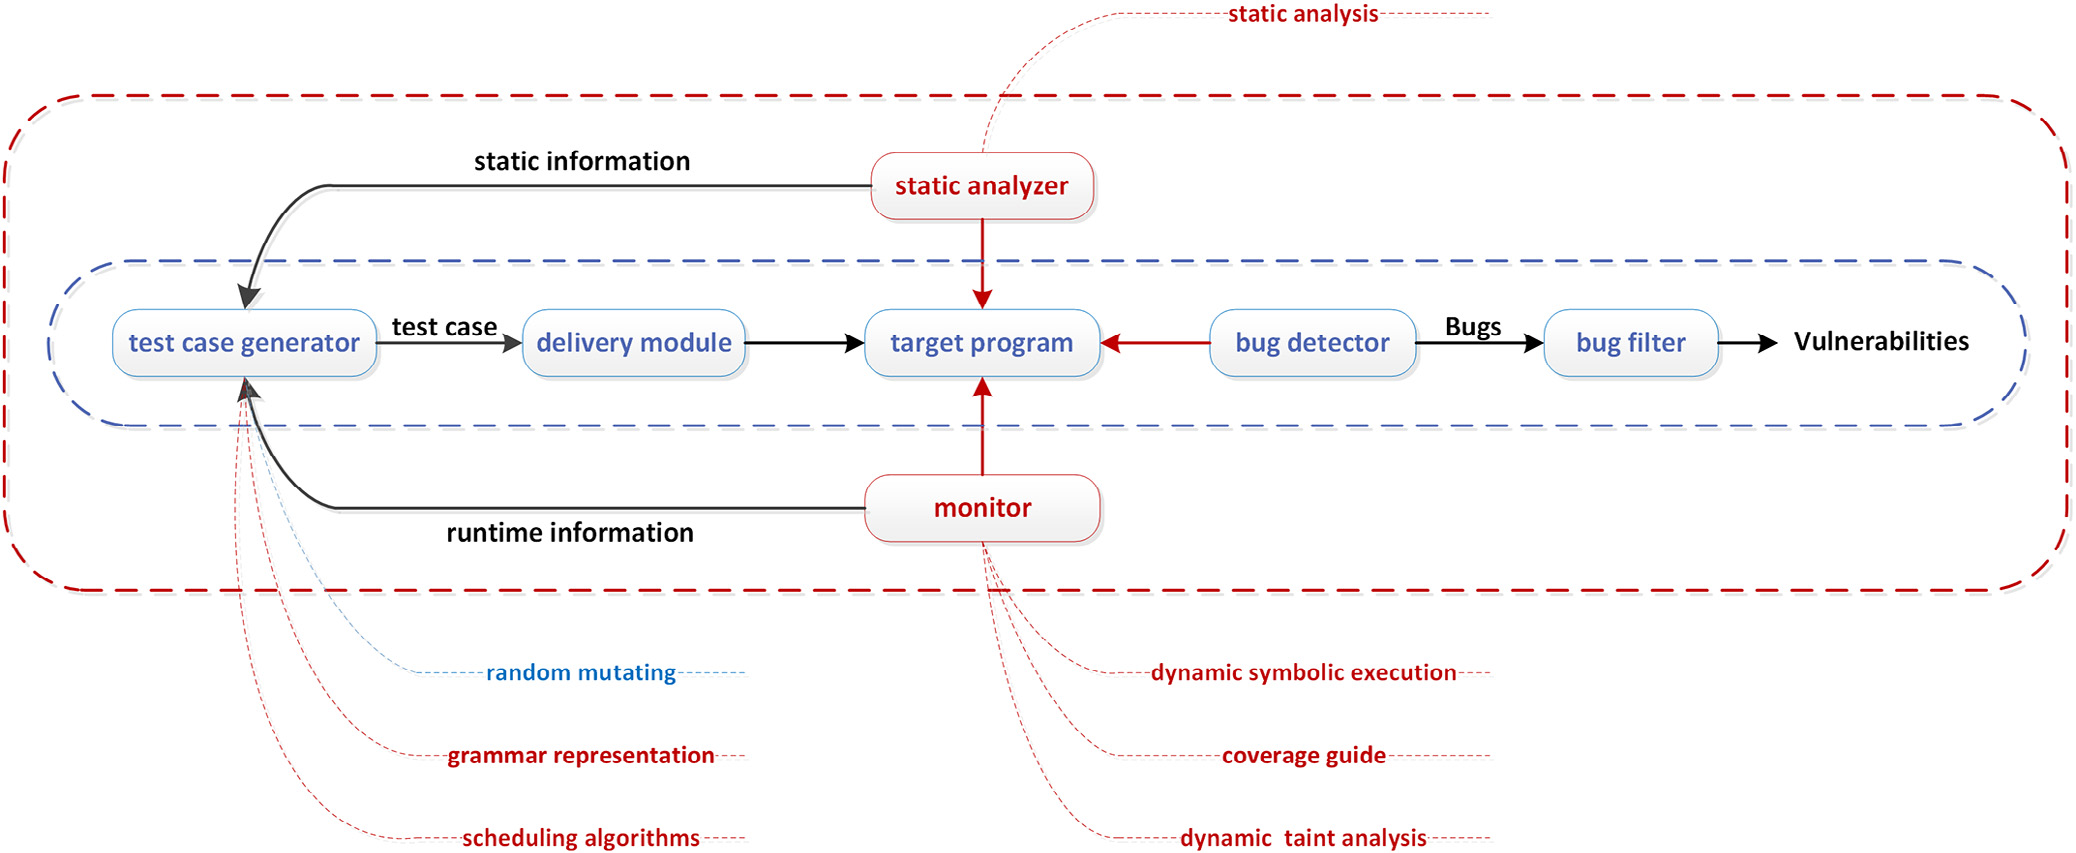
\includegraphics[width=0.9\textwidth]{assets/FuzzingSteps.jpg}
        \caption{Architectural Diagram of a Fuzzing System\cite{Science}}
        \label{fig:FuzzingSteps}
    \end{figure*}
    \subsubsection{Similarities Across Fuzzers}
    Since then, fuzzing systems have become more sophisticated and different techniques have been integrated. However, certain characteristics remain similar between all fuzzing systems. They output some concrete input(s) and configurations that can then be used to reproduce the fuzzer's observation, allowing confirmation, reproduction, and debugging of the discovered issues.\cite{EvaluatingFuzzTesting} They automatically find well-defined bugs, such as assertion errors, divisions by zero, \code{NULL} pointer dereferences, etc.\cite{AllYouEverWanted}

    \subsubsection{Architecture of a Fuzzer}
    \label{ArchitectureFuzzer}
    Figure\ref{fig:FuzzingSteps} shows the architecture of a typical fuzzer. Most fuzzers contain similar parts that are responsible for each step during the fuzzing process. These are explained below

    \paragraph{Target Program}
    The target program (also known as the program under test, or PUT) is the software to be tested. Different fuzzers have different requirements for the type of PUT they support: Some require access to the source code to add instrumentation during compilation, or because they work on an intermediate representation (IR), such as LLVM bytecode.

    \paragraph{Bug Detector}
    The bug detector watches the PUT during execution for illegal states. The simplest implementations trigger on program crashes, more sophisticated bug detectors might check if certain protected parts of the PUT are accessed, for example to check the implemented authentication.

    \paragraph{Bug Filter}
    The list of inputs that put a PUT into an illegal state may contain duplicates, in the sense that they exploit the same software defect. The bug filter attempts to deduplicate this list based on some heuristics such as stack hashes or the order in which basic blocks were executed.

    \paragraph{Test Case Generator}
    The task of the test case generator is to generate and select the next input to be tested. Based on the test case generator, fuzzing systems can be categorized as either mutation-based or generation-based. Mutation-based fuzzers take some inputs to the PUT as their input, and then repeatedly mutate them if the results produce \textquote{interesting} behavior\cite{EvaluatingFuzzTesting}.

    The prioritization is either random or based on a heuristic that assigns a value to each possible next input, which is used to select the next input to pass to the delivery module. Heuristics often take into account information produced by the monitor, such as coverage or distance to target instructions. These approaches can be further combined, for example, by alternating random and heuristic-based input selection.

    \paragraph{Delivery Module}
    The delivery module is responsible for passing the generated test case to the PUT in the expected form and triggering the actual execution. This can be as simple as running a command line utility with specified command line arguments, but can also include creating files to be accessed by the PUT, or even emulating user interaction.

    \paragraph{Monitor}
    Fuzzing systems can be further classified based on how much access the monitor module has to the PUT. Blackbox fuzzers make a single observation: whether or not the PUT has crashed. Graybox fuzzers have limited access to the PUT during execution. Typical information extracted by graybox fuzzers includes which basic blocks were executed in what order, or generally code coverage based on instruction, basic block, or statement. Whitebox fuzzers have full access to the PUT and allow sophisticated reasoning about program structure. Systems that use taint analysis or symbolic execution are categorized as whitebox fuzzers because they deeply examine the program structure during their analysis. Different systems make different tradeoffs, accepting higher analysis costs in the hope of better bug-finding effectiveness.\cite{EvaluatingFuzzTesting}

    \paragraph{Static Analyzer}
    The static analyzer, as its name suggests, attempts to extract information by statically examining the PUT's source code, IR or binary. Such information may include grammars accepted by the PUT or program paths that are considered high risk.

    \subsection{Symbolic Execution}
    \label{SymbolicExecution}
    The concept of symbolic execution in the context of program testing was introduced in \citeyear{Symbex} by \citeauthor{Symbex}.\cite{Symbex} By not executing a PUT with concrete values (such as the number \code{23} or the string \code{"Hello World!"}), but instead modelling certain or all values with mathematical variables, it allows to explore all possible paths of a program. Different engines (such as angr\cite{angr} or Triton\cite{Triton}) allow to perform symbolic execution on source code, an IR or a binary of a PUT.

    \subsubsection{Performing Symbolic Execution}
    During the execution of a given program, a symbolic execution engine computes and updates the so-called symbolic state with each instruction. It contains
    \begin{itemize}
        \item the inputs marked as symbolic as symbols $\alpha_i$,
        \item the symbolic expression store $\sigma$, which in turn contains
        \item symbolic expressions $\phi_j$, which are either a reference to a symbol $\alpha_i$ or an arithmetic combination of symbolic expressions, such as $\phi_j=\phi_k-\phi_l$, and finally
        \item the path constraint $\pi$, which is the conjunction of all branch constraints, i.e. the conditions on symbolic expressions to arrive at a certain point in the program, such as $\phi_1\leq2$ or $\phi_2=\phi_3\land\phi_4=3$.
    \end{itemize}

    During execution, the symbolic state changes according to the specific instruction being executed. If it performs some form of manipulation on existing data, this is represented by adding new symbolic expressions to the symbolic store. If a branch is (not) taken based on a check on variables or registers containing symbolic expressions, the path constraint is extended with an appropriate condition. The exploration of a program can follow different heuristics, such as breath- or depth-first search. Finally, the path constraint collected along certain paths can be formulated as a query to a Satisfiability Modulo Theory (SMT) solver. This solver can then prove whether the path associated with the constraint is reachable with \textit{any} input, and generate an input that directs the PUT execution in exactly the same way as the analyzed execution.

    \subsubsection{Categorizing Symbolic Execution Implementations}
    Symbolic execution implementations can be categorized in several ways: Where static dynamic execution exclusively and exhaustively executes the process described above, dynamic (or concolic, a portmanteau of \textquote{concrete} and \textquote{symbolic}) symbolic execution executes a program symbolically and with concrete values in parallel.

    Online symbolic execution allows multiple paths to be computed in parallel, while offline symbolic execution examines one path at a time. Finally, one can distinguish between partial and full symbolic execution, where only a part or all of the variables and therefore the computation is done symbolically.\cite{Ghidrion}

    \section{Methods}
    \label{Methods}

    Fuzzing is a extensively researched topic. For the search term \textquote{Fuzzing}, Web of Science\cite{WebOfScience} finds 2,741, Scopus\cite{Scopus} finds 2,410, and Google Scholar\cite{GoogleScholar} finds approximately 29,300 works. Even when filtered by the top places, summarizing the current state of symbolic execution in fuzzing from the ground up would be a task beyond the scope of this project.

    However, since fuzzing is such a well-published topic, other researchers have taken on the task of summarizing the state of the art, each group with a slightly different focus. These survey papers can therefore be used to approximate a complete picture of the current state of the art. This is the approach taken by the author of this paper. Section\ref{SurveyPapers} contains a list of the survey papers considered. To ensure accuracy and a consistent level of detail, the works discussed in these survey papers (primary works) are used to confirm or refute how the survey papers discuss the contributions of each primary work. However, the information in the review papers was generally trusted, and an in-depth analysis of each primary paper mentioned was beyond the scope of this work. Therefore, minor inaccuracies may have gone undetected.

    The following rules were applied when selecting review papers for inclusion in this work:
    \begin{itemize}
        \item First, various search engines were used to generate a list of survey papers in the field of fuzzing. Since even the amount of survey papers is overwhelming (Google Scholar\cite{GoogleScholar} returns more than 25,000 results for the search term \textquote{fuzzing survey}), works were only included if their title, abstract, or keywords contained the word section \textquote{fuzz} and if Google Scholar\cite{GoogleScholar} reports that they were cited more than 5 times or if they were published in a high-impact venue.
        \item Then, further review papers discussed, listed, or cited in other review papers were added (such as works listed in \cite{Demystifying}).
        \item Works published before January 1, 2010 (such as\cite{ViolatingAssumptionsWithFuzzing} or\cite{NewTrendsSymbex}) were not included to further limit the scope of this survey.
        \item Then, review papers focusing on a specific technique (such as machine learning\cite{ML1, ML2}) were excluded.
        \item Similarly, review papers focusing on hybrid fuzzing\cite{Hybrid, Exploratory} were discarded, since most hybrid fuzzers use symbolic execution only in a very limited fashion, which negates most of the obstacles faced by classical symbolic execution based fuzzers. However, to provide some introductory insight, a short survey paper on hybrid fuzzing\cite{SurveyHybrid} was selected to be included.
        \item In addition, works focusing on a specific use case for fuzzing, such as testing Internet of Things or other embedded devices\cite{IoT, Embedded, Embedded2}, network protocols\cite{Network, Network2023}, smart contracts\cite{Ethereum}, or JavaScript engines\cite{JavaScript, JavaScript2}, were excluded.
        \item Finally, a selection of additional works were added to the list based on the author's intuition.
    \end{itemize}

    \section{Related Work}
    \label{SurveyPapers}

    This section summarizes contributions of existing survey papers selected as described in Section\ref{Methods} and lists relevant primary works discussed in each. Primary works mentioned without discussion are omitted.

    \papertitle{AllYouEverWanted}
    Using a simple intermediate language (SIMPIL), this paper discusses taint analysis and forward symbolic execution, including examples and analysis of the theoretical foundations of symbolic execution. Although fuzzing is mentioned in several instances, it is not the main focus. However, many of the drawbacks and advantages of fuzzers based on symbolic execution are still listed, and the additional perspective was valuable in compiling this review.

    \papertitle{PreliminaryAssessment}
    After a brief overview of issues faced by symbolic execution based fuzzers, this paper focuses on eight high impact fuzzing tools (JPF-SE and Symbolic (Java) PathFinder\cite{JPFSE, JavaPathFinder}, DART\cite{DART}, CUTE\cite{CUTE} and jCUTE\cite{ExplicitPathModelChecking}, CREST\cite{CREST}, SAGE\cite{SAGE}, Pex\cite{Pex}, EXE\cite{EXE}, and KLEE\cite{KLEE}).

    \papertitle{FuzzingTheStateOfTheArt}
    \citeauthor{FuzzingTheStateOfTheArt} from the Australian Department of Defence provide a comprehensive look at fuzzing - \citetitle{FuzzingTheStateOfTheArt} is the longest of the survey papers discussed. After discussing the taxonomy, concepts, types, and history of fuzzing, the authors discuss a list of 15 papers from the academic literature and ten commercial and open source frameworks. Among these academic papers, they present four papers that employ symbolic execution, namely KLEE\cite{KLEE}, SAGE\cite{SAGE}, GWF\cite{GWF}, and TaintScope\cite{TaintScope}.

    \papertitle{ReviewThreeDecades}
    As the title suggests, this survey paper focuses on symbolic execution. Starting with an explanation of classical symbolic execution, it then provides a list of issues that fuzzing tools based on symbolic execution face, along with attempts to mitigate them by adapting and extending the algorithms. Finally, the authors present five high-impact tools they have worked on: DART\cite{DART}, CUTE\cite{CUTE}, CREST\cite{CREST}, EXE\cite{EXE}, and KLEE\cite{KLEE}.

    \papertitle{Orchestrated}
    Orchestrated surveys \textquote{consist of a collaborative work collecting self-standing sections, each focusing on a key surveyed topic}\cite{Orchestrated}. One of the topics discussed in this particular work is symbolic execution. It includes brief introductions to BBRBP\cite{BBRBP}, AGLT\cite{AGLT}, Darwin\cite{Darwin}, MATRIX RELOADED\cite{MATRIXRELOADED}, and SRA\cite{SRA} in its introduction. As mitigation strategies for path explosion, it discusses SMART\cite{SMART}, DDCSE\cite{DDCSE}, PFA\cite{PFA}, among others. For environment interaction, ASSIE\cite{ASSIE} and Cinger\cite{Cinger} are presented. Finally, to attempt to solve constraints that are too complex for direct invocation of the SMT solver, MCSS\cite{MCSS}, CORAL\cite{CORAL}, and its extension introducing AVM\cite{CORALAVM} are cited.

    \papertitle{Science}
    After discussing the structure of fuzzing systems and different targets observed in literature and industry, this paper focuses on innovations of primary works along the structure of fuzzers. The paper then discusses symbolic execution in the context of the sample generator and the monitor (see Section\ref{ArchitectureFuzzer}). The primary works discussed in this text include CUTE\cite{CUTE}, KLEE\cite{KLEE}, SAGE\cite{SAGE}, TaintScope\cite{TaintScope}, BuzzFuzz\cite{BuzzFuzz}, GWF\cite{GWF}, Dowser\cite{Dowser}, BORG\cite{BORG}, Driller\cite{Driller}, and MoWF\cite{MoWF}. Additionally, the text contains a substantial section comparing symbolic execution based fuzzing systems and their contributions.

    \papertitle{FuzzingASurvey}
    \citeauthor{FuzzingASurvey} focus on coverage-guided fuzzing, mentioning other approaches that can be mixed in and different applications it can be used for. They further broadly discuss the challenges symbolic execution in fuzzing faces. Finally, they present TaintScope\cite{TaintScope} and Driller\cite{Driller} as examples of using symbolic execution for specifically for path exploration.

    \papertitle{FuzzingStateOfTheArt2018}
    The first mention of a symbolic execution based fuzzer in this paper is SAGE\cite{SAGE}, which the authors use to summarize the limitations of whitebox fuzzing. The following section discusses works that advance one step in the fuzzing workflow, including SYMFUZZ\cite{SYMFUZZ}, TaintScope\cite{TaintScope}, and KATCH\cite{KATCH}. Then, and most clearly relevant to this work, \citetitle{FuzzingStateOfTheArt2018} contains a discussion of the limitations of taint analysis and dynamic symbolic execution. Works discussed in this section include SMART\cite{SMART}, HOTG\cite{HigherOrderTestGeneration}, Cloud9\cite{Cloud9}, APLS\cite{APLS}, SAGE\cite{SAGE}, CGF\cite{CGF}, DeepFuzz\cite{DeepFuzz}, TCR\cite{TCR}, DiSE\cite{DiSE}, and CRAXfuzz\cite{CRAXfuzz}.

    \papertitle{EvaluatingFuzzTesting}
    While not a classic survey paper, \citetitle{EvaluatingFuzzTesting} finds issues in how all 32 papers (not listed here for brevity) performed the evaluation of the system they introduced. It further proposes rules to follow to make an evaluation robust. Finally, it contains a list of what advances each paper examined claims to introduce.

    \papertitle{HackArtScience}
    \citeauthor{HackArtScience} gives an easy-to-understand introduction to fuzzing in this work. He distinguishes between blackbox, grammar-based, whitebox, graybox, and hybrid fuzzing, and provides code examples that show how some of these approaches work. In the section on whitebox fuzzing, SAGE\cite{SAGE} is discussed comparatively extensively, KLEE\cite{KLEE}, S2E\cite{S2E}, and SPF\cite{SPF} are mentioned.

    \papertitle{SurveyHybrid}
    This paper focuses on hybrid fuzzing, as the title suggests - the combination of black/greybox and whitebox fuzzing. The discussed works include Hybrid Fuzz Testing\cite{HybridFuzzTesting}, Driller\cite{Driller}, QSYM\cite{QSYM}, SAVIOR\cite{SAVIOR}, and Pangolin\cite{Pangolin}.

    \papertitle{ChallengesAndReflections}
    In comparison to other works, the authors of this article take a less technical and more conceptual approach to surveying the state of the art in fuzzing. They identify areas for improvement, such as usability, residual risk estimation, and fuzzer evaluation techniques, and discuss current approaches and their limitations. To further legitimize their findings, they conducted a survey among security professionals from both academia and industry. The only symbolic execution based fuzzers mentioned are KLEE\cite{KLEE}, SAGE\cite{SAGE}, and Mayhem\cite{Mayhem}.

    \papertitle{ArtScienceEng}
    Beginning with the proposal of a taxonomy for fuzzing itself and the categorization of fuzzers, this paper proposes a general model of fuzzing, explaining the steps and approaches common to fuzzers. It further presents a genealogy, tracing the origins of important works back to the work of \citeauthor{UNIX}. However, it \textquote{does not provide a comprehensive survey on DSE}\cite{ArtScienceEng}, but only discusses whitebox fuzzing in a subsection and refers to other survey papers such as \cite{Orchestrated, AllYouEverWanted} for a more complete overview.

    \papertitle{FuzzingASurveyforRoadmap}
    Similar to what is attempted in this paper, \citetitle{FuzzingASurveyforRoadmap} lists issues along common steps in fuzzing along with attempted solutions, but without the focus on symbolic execution. It includes a short section on symbolic execution in context input search space handling, but discusses very few papers directly, while often mentioning entire families of papers, only some of which rely on symbolic execution.

    \papertitle{FuzzingVulnerabilityDiscoveryTechniques}
    After a short chapter on fuzzer classification, the main focus of this paper is on steps and issues along a typical fuzzer workflow, told through the papers that have made advances in each category. The paper concludes by highlighting current research challenges and suggesting possible approaches. Among the papers discussed are some that rely on symbolic execution: Angora\cite{Angora}, T-FUZZ\cite{TFuzz}, MoWF\cite{MoWF}, and HFL\cite{HFL}.

    \papertitle{SystematicReview2023}
    The authors of this paper guide the reader through advances in fuzzing along the works that introduced them. It includes a section about symbolic execution, which considers the following systems: Driller\cite{Driller}, QSYM\cite{QSYM}, SAVIOR\cite{SAVIOR}, DigFuzz\cite{DigFuzz}, Pangolin\cite{Pangolin}, and QuickFuzz\cite{QuickFuzz}.

    \papertitle{Demystifying}
    This paper dedicates one chapter to explaining the fundamental logic of symbolic execution and then presents three implementations (Driller\cite{Driller}, CONFETTI\cite{CONFETTI}, and FUZZOLIC\cite{FUZZOLIC}). It further examines advances in IoT firmware and kernel fuzzers, but does not explain where the advantages and disadvantages of using symbolic execution in these areas lie.

    \section{Challenges and Mitigation}
    \label{Results}
    This section focuses on attempts to mitigate issues inherent in symbolic execution. It categorizes the challenges and presents a (non-exhaustive) list of works that have introduced some improvement to address them. Many of the listed papers have also implemented more general efficiency improvements, such as SAGE's\cite{SAGE} (and several other papers inspired by it) generational search, which generates multiple new inputs from a single run of the symbolic execution engine by solving the constraint formula with the constraint from each branch flipped independently.

    \subsection{Environment Interactions}
    Within a symbolic execution environment, one can reason about program behavior, but this obviously breaks down when a program contains actions that interact with the real world and cannot be modeled. Examples of this would be unhandled instructions, system calls, interrupts, inter-process communication such as pipes or sockets, or interaction with external systems in general, since they may return unpredictable results because their logic is opaque to the symbolic execution engine.\cite{Demystifying} They may also introduce additional symbolic variables in their return values or have other side effects.

    \paragraph{Concolic Execution}
    For this reason, almost all of the systems examined perform some form of concolic execution. This allows them to simply use the concrete values whenever they encounter instructions that cannot be executed symbolically, acting as an exit whenever no other approach solves a problem. By using concrete values, however, symbolic execution systems sacrifice completeness. But for any system that interacts with the environment in non-trivial ways, this is usually the only way to test it. For non-emulatable function calls, parameters that are not influenceable by inputs — that is, they are not symbolic — are simply used directly, while values for symbolic variables are chosen randomly from the set of solutions to the current constraints on them.\cite{PreliminaryAssessment} In addition, there are further advances that certain systems have made, which mean that they do not have to drop down to concrete values, but can evaluate more logic symbolically.

    \paragraph{Emulating Function Calls}
    One attempt to deal with system calls, common to many symbolic execution engines, is not to perform system calls or even call external libraries, but to present the symbolic execution engine with code that emulates their effects. This preserves the logical integrity of the resulting constraints, and is often more efficient than the original library, since it can rely on the operator's understanding of the function's effect, rather than on how that logic must be transformed to be executable by a machine. Examples of this technique would be EXE\cite{EXE} or KLEE\cite{KLEE}, and all other systems built on top of them (including PYGMALION\cite{PYGMALION}, KATCH\cite{KATCH}, and Cloud9\cite{Cloud9}).

    The downside of this approach is obvious: these summaries must be created, maintained, and tested manually, while fuzzing systems generally strive to require as little operator interaction as possible. There are attempts to automatically infer input-output relational logic in the form of path constraints to be added for complex instructions based on their execution with many different values\cite{ASSIE}. In addition, there are systems that analyze a PUT and prompt the operator to present models only for the parts of the program that actually introduce imprecision, such as Cinger\cite{Cinger}.

    \paragraph{Kernel Fuzzing}
    HFL\cite{HFL} is a kernel fuzzer that relies heavily on symbolic execution. It lists three main issues the authors had to overcome: \textquote{(1) indirect control transfers determined by system call arguments, (2) controlling and matching internal system state via system calls, and (3) nested argument type inference for invoking system calls}\cite{HFL}. To solve these issues, HFL \textquote{(1) converts implicit control transfers to explicit transfers, (2) infers system call sequence to build a consistent system state, and (3) identifies nested arguments types of system calls}\cite{HFL}.

    \subsection{Memory Modelling}
    As described in Section\ref{SymbolicExecution}, symbolic execution engines keep a memory representation of the process in which the PUT is running in memory. However, modelling this memory presents some challenges.

    \paragraph{Arithmetic}
    Operations on a physical machine differ from pure mathematical operations on symbolic expressions. For example, integers can over- or underflow. Modeling floating-point arithmetic is even more difficult because the imprecision introduced by rounding must be accurately represented in the resulting constraints to ensure accuracy of the analysis. These problems are largely solved by symbolic execution engines by representing numbers not as mathematical numbers but as bitmaps, as they would be on the machine. The corresponding constraints must then be added at the bitmap level as well, introducing additional complexity. Certain engines further use special constraint solvers that improve floating-point constraint handling (such as FloPSy\cite{FloPSy}) and complex mathematical constraints (such as CORAL\cite{CORAL} and its extension\cite{CORALAVM}).

    When an instruction performs a jump to a symbolic address, this presents a unique challenge to symbolic execution units, since this single operation increases the size of the program's state space. This is a major scaling problem, to the point of making computation infeasible on all but the most trivial programs. To address this challenge, one may be tempted to simply drop down to a concrete value, as described above, with the discussed drawback of lost completeness, but this is the simplest and most inaccurate way. To maintain more than this base level of accuracy, several strategies have been proposed.

    One such strategy involves separating different operations on symbolic pointers. Although dereferencing a symbolic pointer can be challenging, comparing pointers may still be feasible. Early adopters of this strategy included CUTE\cite{CUTE} and CREST\cite{CREST}, which only consider (in)equality predicates with symbolic pointers. By performing static analysis and solving the constraints on the symbol in question, the amount of valid values it can take can be drastically reduced, thus reducing the number of states that need to be explored.

    EXE\cite{EXE} and KLEE\cite{KLEE} introduced the concept of regarding symbolic pointers as array accesses. An object accessed with a symbolic pointer is copied as often as necessary to model all possible results, including error states. Or, in other words, \textquote{a sound strategy is to consider it a load from any possible satisfying assignment for the expression}\cite{AllYouEverWanted}.

    However, if multiple symbolic pointers access the same data type from different parts of the program, the situation becomes more complex. This is because different pointers might point to different or the same values, thus again creating a scaling problem by introducing many permutations. To address this issue, symbolic execution engines, such as DART\cite{DART}, perform alias analysis at run-time. Alternatively, systems like Vin\cite{BitBlaze} rewrite all memory addresses as scalars based on their name, which is efficient but relies on a potentially unsound assumption of variable name to value equality. Finally, certain SMT solvers (like STP\cite{STP} or Z3\cite{Z3}) can handle alias analysis and can be used to delegate some of the work. This is done by tools such as EXE\cite{EXE}, KLEE\cite{KLEE}, and SAGE\cite{SAGE}.

    \subsection{Path Explosion}
    One of the primary issues that symbolic execution faces is what is known as path explosion. This refers to the fact that the number of program paths is usually exponential with the number of static branches in the code. Since naïve symbolic execution attempts to emulate all possible branches, this requires an unattainable amount of memory and compute resources for all but trivial programs. If the examination is based on a simple depth-first search, it gets stuck in non-terminating loops with symbolic conditions and is therefore rarely used. However, both EXE\cite{EXE} and KLEE\cite{KLEE} can be configured to run in this mode.

    Symbolic execution, when implemented in this way, can inherently help with path explosion by only examining possible branches. An example: When running EXE\cite{EXE} on \code{tcpdump}, only 42\% of the instructions contained symbolic operands, less than 20\% of the symbolic branches have both sides feasible.\cite{EXE}

    One simple approach is to set a user-defined timeout for the symbolic execution engine, after which approaches not based on symbolic execution are used. This is called hybrid fuzzing\cite{HybridFuzzTesting}. It is further discussed in Section\ref{HybridFuzzing}.

    Otherwise, three main strategies are common: reducing the search space, using advanced data structures and other optimizations to delay path explosion, and guiding the search to limit the effects of path explosion.

    \subsubsection{Search Space Reduction}
    Search space reduction can be performed in several ways: First, \textquote{if a program path reaches the same program point with the same symbolic constraints as a previously explored path, then this path will continue to execute exactly the same from that point on and thus can be discarded.}\cite{RWset} This takes advantage of the fact that there are often multiple ways to get to the same program state by performing symbolic state analysis at runtime. Further optimizations based on partial order and symmetry reduction were introduced by \citeauthor{GSE}.\cite{GSE}

    Similarly, MoWF\cite{MoWF} uses knowledge gained by its built-in blackbox fuzzer to prune invalid inputs, thus preventing its symbolic execution engine from getting stuck in input checking and error handling code. CESE\cite{CESE} uses context-free grammars to restrict its symbolic execution engine to interesting paths, as opposed to error handling during parsing. TCR\cite{TCR} intelligently reduces existing test cases and prioritizes the remaining ones according to heuristics to maximize exploration efficiency.

    \subsubsection{Using Advanced Data Structures}
    \label{AdvancedDataStructures}
    \paragraph{State Representation} Since the symbolic state often has only minor differences between closely related paths, it can be represented by a data structure that allows copy-on-write. This means that only the changed parts actually need to be stored, which significantly reduces memory consumption. Many systems use these strategies: KLEE\cite{KLEE}, Mayhem\cite{Mayhem}, S2E\cite{S2E}, BORG\cite{BORG}, and Cloud9\cite{Cloud9}. States can also be statically merged, as in KLEE-FP\cite{KLEEFP}. To further reduce memory pressure, state information can be transferred to disk, as in Mayhem\cite{Mayhem}, BORG\cite{BORG}, and SAGE\cite{SAGE}. The latter also introduced a compact representation for path constraints.\cite{SAGE}

    \paragraph{Function and Data Structure Summaries} To limit the size of paths to be exercised (and thus reduce the amount of symbolic expressions and the size of path constraints), functions can be analyzed and represented by a summary. These summaries can be generated either automatically, as in SMART\cite{SMART}, Higher Order Test Generation\cite{HigherOrderTestGeneration}, or Demand-Driven Compositional Symbolic Execution\cite{DDCSE}, or manually, as described by \citeauthor{PFA}\cite{PFA}. The latter also introduced a system where common complex structures such as strings and regular expressions can be manually transformed into constraints.\cite{PFA} The use of function summaries essentially reduces the problem of interprocedural paths to reasoning about intraprocedural paths. This has been demonstrated in LATEST\cite{LATEST}.

    \subsubsection{Guiding the Execution}
    The approach to mitigating the path explosion problem that has received the most attention is execution guiding. It attempts to direct execution to parts of the PUT that are deemed interesting, in order to complete the analysis (or at least produce findings) as quickly as possible, and before the fuzzer gets stuck and fails to make significant progress.

    Since it is unknowable where exactly findings will be produced, search heuristics of varying complexity are used to select the next input to evaluate. These can take any number of inputs from the program monitor (see Section\ref{ArchitectureFuzzer}) and trade off increased complexity for better precision.

    \paragraph{Dynamic Analysis} Most commonly, symbolic execution based fuzzers guide execution by using the input that increases the instruction, basic block, or statement) coverage of the code. Examples include EXE\cite{EXE}, SAGE\cite{SAGE}, and CREST\cite{CREST}. Complementary, Fitnex\cite{Fitnex} is a state-dependent fitness function that measures the distance between already discovered feasible paths to a given test target (as defined by any other heuristic).

    Other systems reward inputs that lead to longer runtimes, as in Automatic Generation of Load Tests\cite{AGLT}, or those that produce very different outputs based on very similar inputs, as in Symbolic Robustness Analysis\cite{SRA}. QuickFuzz\cite{QuickFuzz} weighs the approximate cost of executing a given path against its demand, and selects the next input based on this ratio.

    \paragraph{Static Analysis} The second group of attempts revolves around static analysis, usually in the form of examining the control flow graph (CFG) of a PUT. CREST\cite{CREST} \textquote{is an extensible platform for building and experimenting with heuristics for selecting paths to explore}\cite{ReviewThreeDecades} and supports analysis of CFGs. This analysis may mark parts of the PUT as interesting based on various criteria and direct the execution towards them. GRT\cite{GRT} and VUzzer\cite{VUzzer} are examples of systems that use general static analysis. The following are examples of more specific static analysis heuristics:

    \begin{itemize}
        \item Directed Incremental Symbolic Execution\cite{DiSE}, Directed Test Suite Augmentation\cite{DTSA}, MATRIX RELOADED\cite{MATRIXRELOADED}, and KATCH\cite{KATCH} direct execution towards code that has changed in a patch, thus using fuzzing as regression testing.
        \item Chopper\cite{Chopped} also uses code differences between two versions of a PUT to steer execution, but reverses the incentive structure: It ignores (or lazily executes) certain functions deemed uninteresting in order to focus on certain parts of the PUT and prevent path explosion. While this could be done manually, Chopper\cite{Chopped} uses a heuristic to mark as uninteresting parts of the PUT that are far away from the code changed in the examined patch.
        \item Darwin\cite{Darwin} uses symbolic execution to generate inputs that are slightly different from crashing inputs, which can then be used to triage and debug a particular software bug.
        \item CRAXfuzz\cite{CRAXfuzz} contains heuristics to identify interesting function calls such as \code{malloc}.
        \item Dowser\cite{Dowser} looks for pointer dereferences in loops.
        \item SAVIOR\cite{SAVIOR} uses UndefinedBehaviorSanitizer\cite{UndefinedBehaviorSanitizer} to find potential bugs.
        \item BORG\cite{BORG} directs the analysis to buffer over-reads.
    \end{itemize}

    Alternatively, the approach can be reversed, working backwards from interesting parts of the PUT to external control structures, as in DrillerGo\cite{DrillerGo}.

    \paragraph{Probabilistic Approaches}
    Recent work has introduced approaches that use heuristics to assign a probability to each potential next input and select which to execute based on that value. DeepFuzz\cite{DeepFuzz} does this with the goal of finding inputs that penetrate deeper into a PUT. MEUZZ\cite{MEUZZ} uses machine learning to examine potential next inputs and uses symbolic execution to validate the results. Finally, DigFuzz\cite{DigFuzz} uses Monte Carlo path optimization to quantify the difficulty of each path using graybox fuzzing, and then lets the whitebox fuzzer focus on the paths that are believed to be the most challenging for graybox fuzzing to make progress.

    \subsection{Constraint Solving}
    \label{ConstraintSolving}
    For most fuzzing systems, constraint solving dominates the runtime. Therefore, it is an area that has received a lot of attention, and several optimizations have been proposed to make query evaluation faster and, in some cases, even possible. They can be categorized as follows

    \subsubsection{Query Optimization}
    \paragraph{Query Splitting} While solving the entire query may not be feasible, solving parts of it often is. This approach can be further divided into two approaches. The first attempts to identify independent sub-queries and solve them independently (implemented in EXE\cite{EXE} and KLEE\cite{KLEE}, among others). This has the obvious limitation that even the smallest independent but internally interdependent parts of the query may still be too large to solve. The second approach (implemented in Mixed Concrete-Symbolic Solving\cite{MCSS}) sacrifices some of its claim to completeness by solving only parts of the query and using the solution to solve the rest. This approach can produce false negatives, where there is a solution but not with the results selected by the solver based on the first query.

    \paragraph{Query Reduction} Symbolic execution often generates inefficient queries for the logic that a particular function or program emulates. By using heuristics such as pattern matching, multiple constraints can be reduced to a single constraint. However, while this approach shrinks the query passed to the SMT solver, it introduces a new scaling problem itself - the optimization passes for complex queries may consume an infeasible amount of time or resources, even to the point where solving the query without optimization is more efficient. Therefore, when introducing such heuristics, systems must carefully balance optimization and SMT solver execution time.

    Optimization can be done either at symbolic execution runtime or afterwards on the complete query. Examples of the former are \textquote{loop-guard patterns matching rules to identify a constraint that defines the number of iterations of input-dependent loops during dynamic symbolic execution, then set new constraints representing the pre- and post-loop conditions to summarize sets of executions of that loop}\cite{Science}, as implemented in SAGE\cite{SAGE}, BORG\cite{BORG}, or APLS\cite{APLS}.

    Alternatively, the use of function summaries (as discussed in Section\ref{AdvancedDataStructures}) can also help to reduce the complexity of SMT queries, since the generated logical relationship between input and output is not bound to the code and therefore to the available instructions. In addition, certain functions can be assigned only partial function summaries if they are called with only certain values, similar to mocks and stubs in unit testing. Moles\cite{Moles} provides a framework for this.

    Finally, in certain contexts it may be advantageous not to use Intermediate Representation (IR) for symbolic execution, but to integrate symbolic emulation with native execution through dynamic binary translation, which avoids additional instructions (since it often takes several RISC instructions in IR to replace one CISC instruction) and allows finer-grained control over the constraint, thus making it smaller. This is done in QSYM\cite{QSYM}.

    \subsubsection{Using Information from Previous Queries}
    \paragraph{Exploiting Query Similarities} Since fuzzing systems based on concolic execution generate the next input based on the path that the PUT executed under the previous input by inverting one of the constraints, there is a strong temporal relationship between successive constraint sets and thus SMT queries. A solution to the first query is obviously known in the form of the input that originally generated the query. To solve the second, very similar query, fuzzing systems can thus use parts of the first solution, since if the part of the query they solved did not change, they might also solve the second query.

    This is a common approach, with subtle differences in implementation: SAGE\cite{SAGE} excludes parts of the query solved by previous results from the query passed to the SMT solver. CUTE\cite{CUTE} relies on a similar mechanism and adds an optimization that supersets of queries often do not invalidate existing solutions. An example of this is when additional checks are performed in the PUT on a particular variable that was previously tested to be a valid input to the function in question further down the stack. Finally, KLEE\cite{KLEE} introduced a more versatile counterexample caching scheme for its SMT queries.

    \paragraph{Advanced Query Relationship Analysis}
    More recently, systems have introduced complex data structures to store their SMT queries, which then allow solvers to efficiently combine information gathered from previous invocations by exploiting the mathematical similarities between queries. Pangolin\cite{Pangolin}, for example, uses polyhedral path abstraction to replace query parts for more efficient models based on previous results.

    \subsubsection{Improved SMT Solvers}
    While some of the improvements discussed above can be implemented in the fuzzers, a whole class of optimizations must be implemented in the SMT solver. For this reason, improved SMT solvers have been developed alongside many of the more influential symbolic execution based fuzzers. Since they are not part of the fuzzing systems themselves, they have not been analyzed as part of this work. Nevertheless, the following SMT solvers are worth mentioning:

    Z3\cite{Z3} is one of the most powerful SMT solvers available today. It is developed at Microsoft and is available as open source under a MIT license and therefore widely used, e.g. in SAGE\cite{SAGE} or angr\cite{angr} (which is used by Driller\cite{Driller}). Other SMT solvers used in symbolic execution based fuzzing are STP\cite{STP}, Yices\cite{Yices}, or cvc5\cite{CVC5} (which was built during the development of EXE\cite{EXE}).

    \subsubsection{Alternatives to SMT Solvers}
    While the approaches listed above may improve the runtime of SMT solvers, they do not solve the fundamental problem of the exponential complexity they face. A set of fuzzers therefore implement systems that allow them to reason about the relationship between input and program execution path without relying on SMT solvers. It can be argued that these systems should no longer be classified as using symbolic execution, since their solutions are often only approximate, but since their fundamental approach is similar, and they are often listed next to symbolic execution based fuzzers in review papers, they are still discussed here.

    Fuzzers that analyse the dependency between input data and the state space, and approximate solutions to path constraints based on this to avoid expensive calls to an SMT solver, are fairly common\cite{WEIZZ}:

    \begin{itemize}
        \item Intriguer\cite{Intriguer} uses taint analysis to detect instructions that access a wide range of input bytes, then performs symbolic execution for those instructions deemed important, invoking the underlying SMT solver only for complicated queries.
        \item Angora\cite{Angora} solves path constraints using a combination of context-sensitive branch coverage, scalable byte-level taint tracking, gradient descent search, input length exploration, and type and shape inference.
        \item Eclipser\cite{Eclipser} uses instrumentation on the PUT to generate partial path conditions, which can then be solved without invoking SMT solvers to generate further input.
        \item SMT formulas can be transformed into programs, which can then be solved using a coverage-guided fuzzer to generate solutions to the initial formula. JFS\cite{JFS} uses this technique to find solutions to floating-point constraints.
        \item REDQUEEN\cite{REDQUEEN} exploits the fact that much of the input data ends up in the state space and uses simple transformations on the input data rather than relying on taint analysis or symbolic execution to bypass checksums.
        \item Other proposals include approximate SMT solvers, such as FUZZY-SAT implemented in FUZZOLOGIC\cite{FUZZOLIC}, or optimistic SMT solvers, such as in QSYM\cite{QSYM}.
    \end{itemize}

    \subsection{Handling Concurrency}
    Testing real-life concurrent programs in general is difficult because of their inherent non-determinism. This is also a challenge for symbolic execution based fuzzers. However, some progress has been made in this area: Generalized Symbolic Execution\cite{GSE} uses model checkers that are able to handle multi-threading (and other forms of non-determinism). In general, \textquote{concolic testing was successfully combined with a variant of partial order reduction to test concurrent programs effectively.\cite{ScalableAutomatedMethods, OpenDistributedPrograms, ExplicitPathModelChecking, RaceDetection}}\cite{ReviewThreeDecades}

    Another development in the area of testing concurrent programs with symbolic execution was introduced in SPIN\cite{SPIN}: It allows checking whether a concurrent program is equivalent to a sequential, less efficient but less error-prone implementation of the same logic. It is used to check complex parallel numerical computations.

    \subsection{Recursive Data Structures}
    Similar to concurrency, recursive data structures are difficult to handle in any test framework. In the area of symbolic execution fuzzers, GSE\cite{GSE} uses lazy initialisation on recursive data structures. Pex\cite{Pex} supports inputs of primitive types as well as complex (i.e. recursive) data types. To handle the latter, Pex analyses the PUT and generates factory methods for each. These invoke a constructor and a sequence of methods whose parameters are also determined by Pex's analysis.

    \subsection{Hybrid Fuzzing}
    \label{HybridFuzzing}
    Hybrid Fuzzing describes systems that combine multiple approaches to improve the effectiveness of fuzzing. Many of these systems include components that make use of symbolic execution. However, because they use symbolic execution selectively, many of the challenges described above are avoided. As described in Section\ref{Methods}, hybrid fuzzing systems have only been tangentially analysed for this thesis. However, to give the reader an introduction, this section discusses a non-exhaustive list of hybrid fuzzing systems.

    \paragraph{Alternating Fuzzing Types} Tools such as Driller\cite{Driller} perform black- or greybox fuzzing (in the case of Driller using AFL\cite{AFLPlusPlus}) until they are \textit{stuck}, i.e. unable to produce inputs that discover additional paths. Driller then, and only then, invokes its concolic execution engine (Driller uses angr\cite{angr}) to trace the program under investigation that was executed with one of the previously generated inputs, and to generate a new input based on the collected path constraint that reaches a section of the PUT that Driller was previously unable to reach. Because Driller does not use symbolic execution as its primary discovery tool, it does not suffer from issues such as path explosion because it only ever executes one path at a time using symbolic execution.

    Other systems that interleave black-/greybox and symbolic execution based fuzzing are Hybrid Concolic Testing\cite{HCT} and Cyberdyne\cite{Cyberdyne}. DrillerGo\cite{DrillerGo} uses a similar approach, but specifically targets \textquote{unsafe system calls or suspicious locations or functions in the call stack of a reported vulnerability that we wish to reproduce}\cite{DrillerGo}. Other targeted hybrid fuzzing systems include 1dVul\cite{1dVul} or BugMiner\cite{BugMiner}.

    \paragraph{PUT Manipulation} By removing code blocks that are deemed irrelevant, T-FUZZ\cite{TFuzz} prevents its mutation-based fuzzer (which does not use symbolic execution) from getting stuck. It then employs symbolic execution to validate the bugs found. TaintScope\cite{TaintScope} uses taint analysis to bypass checksum checks, and then uses symbolic execution to fix checksum fields in malformed test cases. Similarly, Stinger\cite{Stinger} analyses a PUT and then uses symbolic execution only on those parts of the PUT that contribute to path constraints. In this way, the overhead introduced by a symbolic execution engine can be limited to parts of the program.

    \paragraph{High Quality Test Input Generation} IFL\cite{IFL} generates high quality inputs to a smart contract based on a symbolic execution engine and then uses them to train a neural network. This can then be used to fuzz other smart contracts as they often implement similar functionality.

    PYGMALION\cite{PYGMALION} uses symbolic execution to create a grammar from a program, generates valid inputs from this, and finally uses these in fuzzers (AFL\cite{AFLPlusPlus} and KLEE\cite{KLEE}) to measure the code coverage achieved. AUTOGRAM\cite{AUTOGRAM} achieves a similar goal of generating a context-free grammar that a PUT will accept by running it with different inputs based on taint analysis.

    \paragraph{Other Uses of Symbolic Execution} SYMFUZZ\cite{SYMFUZZ} uses symbolic execution to determine the optimal mutation ratio of a given program-seed pair. When a software vendor's program crashes on a customer's device, BBRBP\cite{BBRBP} generates new input that contains no, or at least less, private information. To achieve this, the instructions executed when a program is fed the original crashing input are recorded and then executed using symbolic execution. Finally, the generated path constraint is solved by an SMT solver, which produces a new, unrelated input.

    \section{Future Work}
    \label{FutureWork}
    This work marks only the beginning of what information can be extracted from the combination of review papers and primary works discussed in this work or even in this field in general. What follows is a list of ideas for further analyses.

    \subsection{Additional Review Papers to Consider}
    Section\ref{Methods} mentions different criteria, according to which survey papers were excluded from this work. However, they might still contain important information missed by excluding them. Specifically, certain works appeared to early\cite{AutomaticTestDataGeneration, BruteForceVulnDiscovery,BreakingSoftware}, or focus on symbolic execution based software testing, but do not primarily concern fuzzing\cite{DSETestGeneration, SurveySymbex, SearchStrategies, NewTrendsSymbex, ReviewConcolicTesting}.

    \subsection{Bibliometry}
    Survey papers, taken together, might be a good way of measuring the importance of primary papers. By carefully selecting survey papers, looking at their bibliography and counting how often each primary paper appears, one could get a measure of importance for each. To ensure fairness, the scores would have to be weighted according to how many review papers were only written after their publication date.

    Compared to examining the bibliographies of primary papers, works that introduced a new technique that was copied or adapted by many subsequent papers would likely be weighted less heavily. This would bias the results towards papers that were highly influential because of their results and ongoing development, not just because of the techniques they introduced.

    A time-based analysis might even distinguish between works that are still relevant today, as opposed to those that were superseded soon after publication by other works that implemented the same approach more successfully.

    Finally, analysing the context in which a particular citation appears could further improve the accuracy of a bibliometric score of the importance of a primary work. If it is only mentioned, it could be considered less important than if it is discussed in detail. Instead of complex linguistic analysis, counting the number of times a source is cited or examining the section in which it appears could serve as an imperfect but easier to implement proxy.

    \subsection{Author Analysis}
    While reading the survey papers discussed in Section\ref{SurveyPapers}, one thing that became apparent was that some review papers were (co-)written by authors of important primary works. One example is Cristian Cadar, who is the author of EXE\cite{EXE}, KLEE\cite{KLEE}, KLEE-FP\cite{KLEEFP} RWset\cite{RWset}, KATCH\cite{KATCH}, EGT\cite{EGT}, Chopped\cite{Chopped}, and JFS\cite{JFS} and co-authored the review papers\cite{ReviewThreeDecades, ChallengesAndReflections, PreliminaryAssessment}.

    This is to be expected, as these authors already know the material very well. But it may also mean that their own work is over-represented in the review papers they have helped to compile. Investigating this relationship may provide an insight into how easy or difficult it is to gain recognition as an author new to the field. It may also serve as a measure of how likely it is that innovative work by new authors is overlooked by reviewers.

    \subsection{Genealogy}
    Since most works discussed in this paper introduce improvements in a specific part of a fuzzing system, they often build on an existing system to provide the foundation. For example, PYGMALION\cite{PYGMALION}, KATCH\cite{KATCH}, and Cloud9\cite{Cloud9} build on KLEE\cite{KLEE}, APLS\cite{APLS} extends SAGE\cite{SAGE}, and CRAXfuzz\cite{CRAXfuzz} extends S2E\cite{S2E}, which in turn extends KLEE\cite{KLEE}.

    Building a genealogy tree from the primary works discussed might provide a list of highly adaptable and stable projects, which in turn might be more suitable for deployment in commercial applications. \citetitle{ArtScienceEng}\cite{ArtScienceEng} contains a diagram of such a genealogy. However, as this work does not focus on symbolic execution based fuzzing, it does not distinguish nuances within this subfield and only includes a limited number of projects, while \citetitle{Hybrid}\cite{Hybrid} focuses on hybrid fuzzing systems only.

    In addition, if not extending the code itself, ideas or concepts introduced by one paper may be copied or adapted by subsequent work. Building a genealogical dataset across these may reveal hidden relationships between projects and show the importance of ideas implemented in fuzzers across the board.

    \subsection{Meta Survey}
    Finally, one could compare review papers based on different categories: primary works discussed (see above), categorisations of fuzzers, or more specifically, categorisations of problems that symbolic execution faces in fuzzing and the solutions to them that different works propose.
    \section{Conclusion}

    \label{Conclusion}
    This survey provides an introduction to fuzzing, in particular the use of symbolic execution in fuzzing systems, its challenges and innovations. It presents a discussion of the theoretical underpinnings of both fuzzing in general and symbolic execution in particular, and explains how these two approaches to software testing have been combined to create state-of-the-art systems.

    As this area has received considerable attention from both academia and industry, fuzzing survey papers are used to collect significant works, including summaries and discussions of them. First, the focus of each of the 17 selected survey papers is summarised, along with a list of 78 discussed symbolic execution based fuzzers. The latter are then combined, extended and categorised. The resulting list shows that a diverse set of attempts has been made to mitigate each of the inherent challenges of symbolic execution, thus making it applicable to real-world programs.

    Finally, this work reflects on its own approach of using existing survey papers to gather information about a particular area. Both the limitations of this process and possible additions to this work are discussed. By using this approach, an otherwise unfeasibly large area of research has been explored, providing a comprehensive overview of the state of the art in symbolic execution based fuzzing.

    \defbibheading{bibliography}[\bibname]{\section*{#1}}
    \addcontentsline{toc}{section}{\bibname}
    \printbibliography

    % \renewcommand{\thesubsection}{\arabic{subsection}}
    % \renewcommand{\thesubsubsection}{\arabic{subsection}.\arabic{subsubsection}}
    % \setcounter{subsection}{0}
    % \setcounter{subsubsection}{0}
    % \section*{Appendix}
    % \addcontentsline{toc}{section}{Appendix}
\end{multicols}

\end{document}
